\documentclass[twoside]{book}

% Packages required by doxygen
\usepackage{fixltx2e}
\usepackage{calc}
\usepackage{doxygen}
\usepackage[export]{adjustbox} % also loads graphicx
\usepackage{graphicx}
\usepackage[utf8]{inputenc}
\usepackage{makeidx}
\usepackage{multicol}
\usepackage{multirow}
\PassOptionsToPackage{warn}{textcomp}
\usepackage{textcomp}
\usepackage[nointegrals]{wasysym}
\usepackage[table]{xcolor}

% Font selection
\usepackage[T1]{fontenc}
\usepackage[scaled=.90]{helvet}
\usepackage{courier}
\usepackage{amssymb}
\usepackage{sectsty}
\renewcommand{\familydefault}{\sfdefault}
\allsectionsfont{%
  \fontseries{bc}\selectfont%
  \color{darkgray}%
}
\renewcommand{\DoxyLabelFont}{%
  \fontseries{bc}\selectfont%
  \color{darkgray}%
}
\newcommand{\+}{\discretionary{\mbox{\scriptsize$\hookleftarrow$}}{}{}}

% Page & text layout
\usepackage{geometry}
\geometry{%
  a4paper,%
  top=2.5cm,%
  bottom=2.5cm,%
  left=2.5cm,%
  right=2.5cm%
}
\tolerance=750
\hfuzz=15pt
\hbadness=750
\setlength{\emergencystretch}{15pt}
\setlength{\parindent}{0cm}
\setlength{\parskip}{3ex plus 2ex minus 2ex}
\makeatletter
\renewcommand{\paragraph}{%
  \@startsection{paragraph}{4}{0ex}{-1.0ex}{1.0ex}{%
    \normalfont\normalsize\bfseries\SS@parafont%
  }%
}
\renewcommand{\subparagraph}{%
  \@startsection{subparagraph}{5}{0ex}{-1.0ex}{1.0ex}{%
    \normalfont\normalsize\bfseries\SS@subparafont%
  }%
}
\makeatother

% Headers & footers
\usepackage{fancyhdr}
\pagestyle{fancyplain}
\fancyhead[LE]{\fancyplain{}{\bfseries\thepage}}
\fancyhead[CE]{\fancyplain{}{}}
\fancyhead[RE]{\fancyplain{}{\bfseries\leftmark}}
\fancyhead[LO]{\fancyplain{}{\bfseries\rightmark}}
\fancyhead[CO]{\fancyplain{}{}}
\fancyhead[RO]{\fancyplain{}{\bfseries\thepage}}
\fancyfoot[LE]{\fancyplain{}{}}
\fancyfoot[CE]{\fancyplain{}{}}
\fancyfoot[RE]{\fancyplain{}{\bfseries\scriptsize Generated by Doxygen }}
\fancyfoot[LO]{\fancyplain{}{\bfseries\scriptsize Generated by Doxygen }}
\fancyfoot[CO]{\fancyplain{}{}}
\fancyfoot[RO]{\fancyplain{}{}}
\renewcommand{\footrulewidth}{0.4pt}
\renewcommand{\chaptermark}[1]{%
  \markboth{#1}{}%
}
\renewcommand{\sectionmark}[1]{%
  \markright{\thesection\ #1}%
}

% Indices & bibliography
\usepackage{natbib}
\usepackage[titles]{tocloft}
\setcounter{tocdepth}{3}
\setcounter{secnumdepth}{5}
\makeindex

% Hyperlinks (required, but should be loaded last)
\usepackage{ifpdf}
\ifpdf
  \usepackage[pdftex,pagebackref=true]{hyperref}
\else
  \usepackage[ps2pdf,pagebackref=true]{hyperref}
\fi
\hypersetup{%
  colorlinks=true,%
  linkcolor=blue,%
  citecolor=blue,%
  unicode%
}

% Custom commands
\newcommand{\clearemptydoublepage}{%
  \newpage{\pagestyle{empty}\cleardoublepage}%
}

\usepackage{caption}
\captionsetup{labelsep=space,justification=centering,font={bf},singlelinecheck=off,skip=4pt,position=top}

%===== C O N T E N T S =====

\begin{document}

% Titlepage & ToC
\hypersetup{pageanchor=false,
             bookmarksnumbered=true,
             pdfencoding=unicode
            }
\pagenumbering{alph}
\begin{titlepage}
\vspace*{7cm}
\begin{center}%
{\Large Core\+Interface }\\
\vspace*{1cm}
{\large Generated by Doxygen 1.8.14}\\
\end{center}
\end{titlepage}
\clearemptydoublepage
\pagenumbering{roman}
\tableofcontents
\clearemptydoublepage
\pagenumbering{arabic}
\hypersetup{pageanchor=true}

%--- Begin generated contents ---
\chapter{R\+E\+A\+D\+ME}
\label{md_README}
\Hypertarget{md_README}
\href{https://api.travis-ci.org/symbiote-h2020/CoreInterface}{\tt } \href{https://codecov.io/github/symbiote-h2020/CoreInterface}{\tt }

\section*{Core\+Interface}
\chapter{Class Index}
\section{Class List}
Here are the classes, structs, unions and interfaces with brief descriptions\+:\begin{DoxyCompactList}
\item\contentsline{section}{\hyperlink{classeu_1_1h2020_1_1symbiote_1_1CoreInterfaceApplication}{eu.\+h2020.\+symbiote.\+Core\+Interface\+Application} }{\pageref{classeu_1_1h2020_1_1symbiote_1_1CoreInterfaceApplication}}{}
\item\contentsline{section}{\hyperlink{classeu_1_1h2020_1_1symbiote_1_1controllers_1_1CoreInterfaceController}{eu.\+h2020.\+symbiote.\+controllers.\+Core\+Interface\+Controller} }{\pageref{classeu_1_1h2020_1_1symbiote_1_1controllers_1_1CoreInterfaceController}}{}
\item\contentsline{section}{\hyperlink{classeu_1_1h2020_1_1symbiote_1_1model_1_1QueryRequest}{eu.\+h2020.\+symbiote.\+model.\+Query\+Request} }{\pageref{classeu_1_1h2020_1_1symbiote_1_1model_1_1QueryRequest}}{}
\item\contentsline{section}{\hyperlink{classeu_1_1h2020_1_1symbiote_1_1communication_1_1RabbitManager}{eu.\+h2020.\+symbiote.\+communication.\+Rabbit\+Manager} }{\pageref{classeu_1_1h2020_1_1symbiote_1_1communication_1_1RabbitManager}}{}
\item\contentsline{section}{\hyperlink{classeu_1_1h2020_1_1symbiote_1_1model_1_1Resource}{eu.\+h2020.\+symbiote.\+model.\+Resource} }{\pageref{classeu_1_1h2020_1_1symbiote_1_1model_1_1Resource}}{}
\item\contentsline{section}{\hyperlink{classeu_1_1h2020_1_1symbiote_1_1model_1_1ResourceUrlsRequest}{eu.\+h2020.\+symbiote.\+model.\+Resource\+Urls\+Request} }{\pageref{classeu_1_1h2020_1_1symbiote_1_1model_1_1ResourceUrlsRequest}}{}
\end{DoxyCompactList}

\chapter{Class Documentation}
\hypertarget{classeu_1_1h2020_1_1symbiote_1_1CoreInterfaceApplication}{}\section{eu.\+h2020.\+symbiote.\+Core\+Interface\+Application Class Reference}
\label{classeu_1_1h2020_1_1symbiote_1_1CoreInterfaceApplication}\index{eu.\+h2020.\+symbiote.\+Core\+Interface\+Application@{eu.\+h2020.\+symbiote.\+Core\+Interface\+Application}}


Collaboration diagram for eu.\+h2020.\+symbiote.\+Core\+Interface\+Application\+:
\nopagebreak
\begin{figure}[H]
\begin{center}
\leavevmode
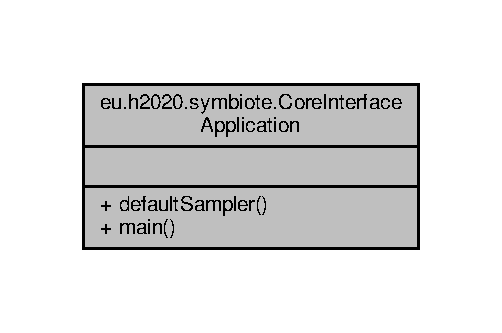
\includegraphics[width=241pt]{classeu_1_1h2020_1_1symbiote_1_1CoreInterfaceApplication__coll__graph}
\end{center}
\end{figure}
\subsection*{Classes}
\begin{DoxyCompactItemize}
\item 
class {\bfseries C\+LR}
\end{DoxyCompactItemize}
\subsection*{Public Member Functions}
\begin{DoxyCompactItemize}
\item 
Always\+Sampler {\bfseries default\+Sampler} ()\hypertarget{classeu_1_1h2020_1_1symbiote_1_1CoreInterfaceApplication_a471bb0daa5bb1e4f52cdca00b81fae69}{}\label{classeu_1_1h2020_1_1symbiote_1_1CoreInterfaceApplication_a471bb0daa5bb1e4f52cdca00b81fae69}

\end{DoxyCompactItemize}
\subsection*{Static Public Member Functions}
\begin{DoxyCompactItemize}
\item 
static void {\bfseries main} (String\mbox{[}$\,$\mbox{]} args)\hypertarget{classeu_1_1h2020_1_1symbiote_1_1CoreInterfaceApplication_a7c7036fb52bab67977fa57f6200b0b7e}{}\label{classeu_1_1h2020_1_1symbiote_1_1CoreInterfaceApplication_a7c7036fb52bab67977fa57f6200b0b7e}

\end{DoxyCompactItemize}


\subsection{Detailed Description}
Core Interface module\textquotesingle{}s entry point. 

Core Interface is a northbound interface for accessing symb\+Io\+Te platform. It allows users (mostly application developers) to query registered resourced and get their U\+R\+Ls. 

The documentation for this class was generated from the following file\+:\begin{DoxyCompactItemize}
\item 
src/main/java/eu/h2020/symbiote/Core\+Interface\+Application.\+java\end{DoxyCompactItemize}

\hypertarget{classeu_1_1h2020_1_1symbiote_1_1controllers_1_1CoreInterfaceController}{}\section{eu.\+h2020.\+symbiote.\+controllers.\+Core\+Interface\+Controller Class Reference}
\label{classeu_1_1h2020_1_1symbiote_1_1controllers_1_1CoreInterfaceController}\index{eu.\+h2020.\+symbiote.\+controllers.\+Core\+Interface\+Controller@{eu.\+h2020.\+symbiote.\+controllers.\+Core\+Interface\+Controller}}


Collaboration diagram for eu.\+h2020.\+symbiote.\+controllers.\+Core\+Interface\+Controller\+:
\nopagebreak
\begin{figure}[H]
\begin{center}
\leavevmode
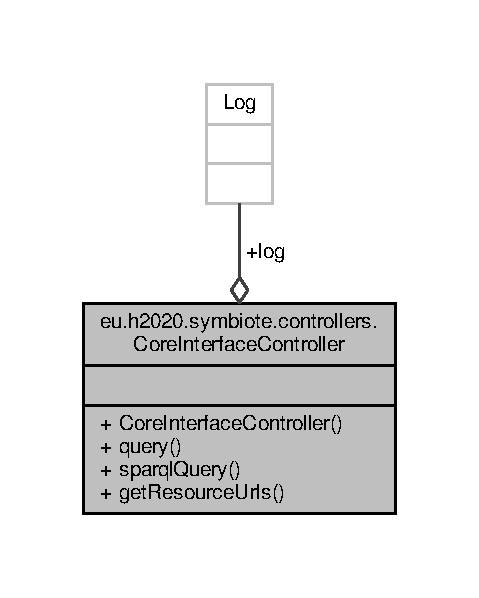
\includegraphics[width=230pt]{classeu_1_1h2020_1_1symbiote_1_1controllers_1_1CoreInterfaceController__coll__graph}
\end{center}
\end{figure}
\subsection*{Public Member Functions}
\begin{DoxyCompactItemize}
\item 
\hyperlink{classeu_1_1h2020_1_1symbiote_1_1controllers_1_1CoreInterfaceController_a58b26a72b6964d21f04c7f680640dcce}{Core\+Interface\+Controller} (\hyperlink{classeu_1_1h2020_1_1symbiote_1_1communication_1_1RabbitManager}{Rabbit\+Manager} rabbit\+Manager)
\item 
Response\+Entity$<$?$>$ \hyperlink{classeu_1_1h2020_1_1symbiote_1_1controllers_1_1CoreInterfaceController_a77e06f47bb9cea92496704aae1b88b86}{query} (@Request\+Param(value=\char`\"{}platform\+\_\+id\char`\"{}, required=false) String platform\+Id,@Request\+Param(value=\char`\"{}platform\+\_\+name\char`\"{}, required=false) String platform\+Name,@Request\+Param(value=\char`\"{}owner\char`\"{}, required=false) String owner,@Request\+Param(value=\char`\"{}name\char`\"{}, required=false) String name,@Request\+Param(value=\char`\"{}id\char`\"{}, required=false) String id,@Request\+Param(value=\char`\"{}description\char`\"{}, required=false) String description,@Request\+Param(value=\char`\"{}location\+\_\+name\char`\"{}, required=false) String location\+\_\+name,@Request\+Param(value=\char`\"{}location\+\_\+lat\char`\"{}, required=false) Double location\+\_\+lat,@Request\+Param(value=\char`\"{}location\+\_\+long\char`\"{}, required=false) Double location\+\_\+long,@Request\+Param(value=\char`\"{}max\+\_\+distance\char`\"{}, required=false) Integer max\+\_\+distance,@Request\+Param(value=\char`\"{}observed\+\_\+property\char`\"{}, required=false) String\mbox{[}$\,$\mbox{]} observed\+\_\+property)
\item 
Response\+Entity$<$?$>$ \hyperlink{classeu_1_1h2020_1_1symbiote_1_1controllers_1_1CoreInterfaceController_adfa6e88c052cd6e8978294588fe116d5}{sparql\+Query} (@Request\+Body String sparql\+Query)
\item 
Response\+Entity$<$?$>$ \hyperlink{classeu_1_1h2020_1_1symbiote_1_1controllers_1_1CoreInterfaceController_a11f9875a81bc3f2a8150b1fb12285ce4}{get\+Resource\+Urls} (@Request\+Param(\char`\"{}id\char`\"{}) String\mbox{[}$\,$\mbox{]} resource\+Id)
\end{DoxyCompactItemize}
\subsection*{Static Public Attributes}
\begin{DoxyCompactItemize}
\item 
static Log {\bfseries log} = Log\+Factory.\+get\+Log(Core\+Interface\+Controller.\+class)\hypertarget{classeu_1_1h2020_1_1symbiote_1_1controllers_1_1CoreInterfaceController_a0890e1d907ac6cfdd976c53c5cdb5743}{}\label{classeu_1_1h2020_1_1symbiote_1_1controllers_1_1CoreInterfaceController_a0890e1d907ac6cfdd976c53c5cdb5743}

\end{DoxyCompactItemize}


\subsection{Detailed Description}
Class defining all R\+E\+ST endpoints. 

Core\+Interface, as the name suggests, is just an interface, therefore it forwards all requests to modules responsible for handling them via Rabbit\+MQ. 

\subsection{Constructor \& Destructor Documentation}
\index{eu\+::h2020\+::symbiote\+::controllers\+::\+Core\+Interface\+Controller@{eu\+::h2020\+::symbiote\+::controllers\+::\+Core\+Interface\+Controller}!Core\+Interface\+Controller@{Core\+Interface\+Controller}}
\index{Core\+Interface\+Controller@{Core\+Interface\+Controller}!eu\+::h2020\+::symbiote\+::controllers\+::\+Core\+Interface\+Controller@{eu\+::h2020\+::symbiote\+::controllers\+::\+Core\+Interface\+Controller}}
\subsubsection[{\texorpdfstring{Core\+Interface\+Controller(\+Rabbit\+Manager rabbit\+Manager)}{CoreInterfaceController(RabbitManager rabbitManager)}}]{\setlength{\rightskip}{0pt plus 5cm}eu.\+h2020.\+symbiote.\+controllers.\+Core\+Interface\+Controller.\+Core\+Interface\+Controller (
\begin{DoxyParamCaption}
\item[{{\bf Rabbit\+Manager}}]{rabbit\+Manager}
\end{DoxyParamCaption}
)}\hypertarget{classeu_1_1h2020_1_1symbiote_1_1controllers_1_1CoreInterfaceController_a58b26a72b6964d21f04c7f680640dcce}{}\label{classeu_1_1h2020_1_1symbiote_1_1controllers_1_1CoreInterfaceController_a58b26a72b6964d21f04c7f680640dcce}
Class constructor which autowires Rabbit\+Manager bean.


\begin{DoxyParams}{Parameters}
{\em rabbit\+Manager} & Rabbit\+Manager bean \\
\hline
\end{DoxyParams}


\subsection{Member Function Documentation}
\index{eu\+::h2020\+::symbiote\+::controllers\+::\+Core\+Interface\+Controller@{eu\+::h2020\+::symbiote\+::controllers\+::\+Core\+Interface\+Controller}!get\+Resource\+Urls@{get\+Resource\+Urls}}
\index{get\+Resource\+Urls@{get\+Resource\+Urls}!eu\+::h2020\+::symbiote\+::controllers\+::\+Core\+Interface\+Controller@{eu\+::h2020\+::symbiote\+::controllers\+::\+Core\+Interface\+Controller}}
\subsubsection[{\texorpdfstring{get\+Resource\+Urls("@Request\+Param(""id"") String[] resource\+Id)}{getResourceUrls(@RequestParam("id") String[] resourceId)}}]{\setlength{\rightskip}{0pt plus 5cm}Response\+Entity$<$?$>$ eu.\+h2020.\+symbiote.\+controllers.\+Core\+Interface\+Controller.\+get\+Resource\+Urls (
\begin{DoxyParamCaption}
\item[{@Request\+Param(\char`\"{}id\char`\"{}) String\mbox{[}$\,$\mbox{]}}]{resource\+Id}
\end{DoxyParamCaption}
)}\hypertarget{classeu_1_1h2020_1_1symbiote_1_1controllers_1_1CoreInterfaceController_a11f9875a81bc3f2a8150b1fb12285ce4}{}\label{classeu_1_1h2020_1_1symbiote_1_1controllers_1_1CoreInterfaceController_a11f9875a81bc3f2a8150b1fb12285ce4}
Endpoint for querying U\+RL of resources\textquotesingle{} Interworking Interface.

After receiving query results, user (or application) may choose interesting resources to contact, but it does not have any means of communicate with resources\textquotesingle{} Interworking Interface. Therefore, it needs to send another request querying for U\+R\+Ls Interworking Services of resources of specified I\+Ds.


\begin{DoxyParams}{Parameters}
{\em resource\+Id} & ID of a resource to get Interworking Interface U\+RL; multiple I\+Ds can be passed\\
\hline
\end{DoxyParams}
\begin{DoxyReturn}{Returns}
map containing entries in a form of \{\char`\"{}resource\+Id1\char`\"{}\+:\char`\"{}\+Interworking\+Interface\+Url1\char`\"{}, \char`\"{}resource\+Id2\char`\"{}\+:\char`\"{}\+Interworking\+Interface2\char`\"{}, ... \} 
\end{DoxyReturn}
\index{eu\+::h2020\+::symbiote\+::controllers\+::\+Core\+Interface\+Controller@{eu\+::h2020\+::symbiote\+::controllers\+::\+Core\+Interface\+Controller}!query@{query}}
\index{query@{query}!eu\+::h2020\+::symbiote\+::controllers\+::\+Core\+Interface\+Controller@{eu\+::h2020\+::symbiote\+::controllers\+::\+Core\+Interface\+Controller}}
\subsubsection[{\texorpdfstring{query("@Request\+Param(value=""platform\+\_\+id"", required=false) String platform\+Id,"@Request\+Param(value=""platform\+\_\+name"", required=false) String platform\+Name,"@Request\+Param(value=""owner"", required=false) String owner,"@Request\+Param(value=""name"", required=false) String name,"@Request\+Param(value=""id"", required=false) String id,"@Request\+Param(value=""description"", required=false) String description,"@Request\+Param(value=""location\+\_\+name"", required=false) String location\+\_\+name,"@Request\+Param(value=""location\+\_\+lat"", required=false) Double location\+\_\+lat,"@Request\+Param(value=""location\+\_\+long"", required=false) Double location\+\_\+long,"@Request\+Param(value=""max\+\_\+distance"", required=false) Integer max\+\_\+distance,"@Request\+Param(value=""observed\+\_\+property"", required=false) String[] observed\+\_\+property)}{query(@RequestParam(value="platform_id", required=false) String platformId,@RequestParam(value="platform_name", required=false) String platformName,@RequestParam(value="owner", required=false) String owner,@RequestParam(value="name", required=false) String name,@RequestParam(value="id", required=false) String id,@RequestParam(value="description", required=false) String description,@RequestParam(value="location_name", required=false) String location_name,@RequestParam(value="location_lat", required=false) Double location_lat,@RequestParam(value="location_long", required=false) Double location_long,@RequestParam(value="max_distance", required=false) Integer max_distance,@RequestParam(value="observed_property", required=false) String[] observed_property)}}]{\setlength{\rightskip}{0pt plus 5cm}Response\+Entity$<$?$>$ eu.\+h2020.\+symbiote.\+controllers.\+Core\+Interface\+Controller.\+query (
\begin{DoxyParamCaption}
\item[{@Request\+Param(value=\char`\"{}platform\+\_\+id\char`\"{}, required=false) String}]{platform\+Id, }
\item[{@Request\+Param(value=\char`\"{}platform\+\_\+name\char`\"{}, required=false) String}]{platform\+Name, }
\item[{@Request\+Param(value=\char`\"{}owner\char`\"{}, required=false) String}]{owner, }
\item[{@Request\+Param(value=\char`\"{}name\char`\"{}, required=false) String}]{name, }
\item[{@Request\+Param(value=\char`\"{}id\char`\"{}, required=false) String}]{id, }
\item[{@Request\+Param(value=\char`\"{}description\char`\"{}, required=false) String}]{description, }
\item[{@Request\+Param(value=\char`\"{}location\+\_\+name\char`\"{}, required=false) String}]{location\+\_\+name, }
\item[{@Request\+Param(value=\char`\"{}location\+\_\+lat\char`\"{}, required=false) Double}]{location\+\_\+lat, }
\item[{@Request\+Param(value=\char`\"{}location\+\_\+long\char`\"{}, required=false) Double}]{location\+\_\+long, }
\item[{@Request\+Param(value=\char`\"{}max\+\_\+distance\char`\"{}, required=false) Integer}]{max\+\_\+distance, }
\item[{@Request\+Param(value=\char`\"{}observed\+\_\+property\char`\"{}, required=false) String\mbox{[}$\,$\mbox{]}}]{observed\+\_\+property}
\end{DoxyParamCaption}
)}\hypertarget{classeu_1_1h2020_1_1symbiote_1_1controllers_1_1CoreInterfaceController_a77e06f47bb9cea92496704aae1b88b86}{}\label{classeu_1_1h2020_1_1symbiote_1_1controllers_1_1CoreInterfaceController_a77e06f47bb9cea92496704aae1b88b86}
Endpoint for querying registered resources. Query parameters are passed via G\+ET request params and are all optional. When passing multiple parameters, including multiple observed\+\_\+properties, they are all linked with logical A\+ND operator. In \char`\"{}text\char`\"{} parameters (name, description, platform\+Name, owner, location\+Name), $\ast$ can be used as a wildcard in the beginning or/and in the end of value.


\begin{DoxyParams}{Parameters}
{\em platform\+Id} & symb\+Io\+Te ID of a platform that resource belongs to \\
\hline
{\em platform\+Name} & name of a platform that resource belongs to \\
\hline
{\em owner} & owner of the resource \\
\hline
{\em name} & name of the resource \\
\hline
{\em id} & symb\+Io\+Te ID of the resource \\
\hline
{\em description} & description of the resource \\
\hline
{\em location\+\_\+name} & name of resource location \\
\hline
{\em location\+\_\+lat} & latitude of resource location \\
\hline
{\em location\+\_\+long} & longitude of resource location \\
\hline
{\em max\+\_\+distance} & maximal distance from specified resource latitude and longitude (in meters) \\
\hline
{\em observed\+\_\+property} & property observed by resource; can be set multiple times to indicate more than one observed property \\
\hline
\end{DoxyParams}
\begin{DoxyReturn}{Returns}
query result as body or null along with appropriate error H\+T\+TP status code 
\end{DoxyReturn}
\index{eu\+::h2020\+::symbiote\+::controllers\+::\+Core\+Interface\+Controller@{eu\+::h2020\+::symbiote\+::controllers\+::\+Core\+Interface\+Controller}!sparql\+Query@{sparql\+Query}}
\index{sparql\+Query@{sparql\+Query}!eu\+::h2020\+::symbiote\+::controllers\+::\+Core\+Interface\+Controller@{eu\+::h2020\+::symbiote\+::controllers\+::\+Core\+Interface\+Controller}}
\subsubsection[{\texorpdfstring{sparql\+Query("@Request\+Body String sparql\+Query)}{sparqlQuery(@RequestBody String sparqlQuery)}}]{\setlength{\rightskip}{0pt plus 5cm}Response\+Entity$<$?$>$ eu.\+h2020.\+symbiote.\+controllers.\+Core\+Interface\+Controller.\+sparql\+Query (
\begin{DoxyParamCaption}
\item[{@Request\+Body String}]{sparql\+Query}
\end{DoxyParamCaption}
)}\hypertarget{classeu_1_1h2020_1_1symbiote_1_1controllers_1_1CoreInterfaceController_adfa6e88c052cd6e8978294588fe116d5}{}\label{classeu_1_1h2020_1_1symbiote_1_1controllers_1_1CoreInterfaceController_adfa6e88c052cd6e8978294588fe116d5}
Endpoint for querying registered resources using S\+P\+A\+R\+QL. 

Currently not implemented. 

The documentation for this class was generated from the following file\+:\begin{DoxyCompactItemize}
\item 
src/main/java/eu/h2020/symbiote/controllers/Core\+Interface\+Controller.\+java\end{DoxyCompactItemize}

\hypertarget{classeu_1_1h2020_1_1symbiote_1_1communication_1_1RabbitManager}{}\section{eu.\+h2020.\+symbiote.\+communication.\+Rabbit\+Manager Class Reference}
\label{classeu_1_1h2020_1_1symbiote_1_1communication_1_1RabbitManager}\index{eu.\+h2020.\+symbiote.\+communication.\+Rabbit\+Manager@{eu.\+h2020.\+symbiote.\+communication.\+Rabbit\+Manager}}


Collaboration diagram for eu.\+h2020.\+symbiote.\+communication.\+Rabbit\+Manager\+:
\nopagebreak
\begin{figure}[H]
\begin{center}
\leavevmode
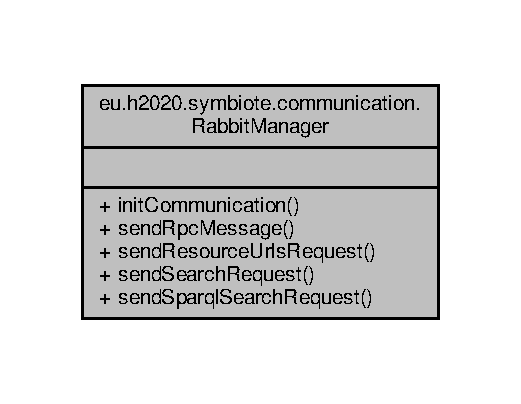
\includegraphics[width=250pt]{classeu_1_1h2020_1_1symbiote_1_1communication_1_1RabbitManager__coll__graph}
\end{center}
\end{figure}
\subsection*{Public Member Functions}
\begin{DoxyCompactItemize}
\item 
void \hyperlink{classeu_1_1h2020_1_1symbiote_1_1communication_1_1RabbitManager_a30abf6a670122eb22a8105a206858616}{init\+Communication} ()
\item 
String \hyperlink{classeu_1_1h2020_1_1symbiote_1_1communication_1_1RabbitManager_a9c71bf18d0bf371fd35c977a69861855}{send\+Rpc\+Message} (String exchange\+Name, String routing\+Key, String message, String class\+Type)
\item 
Map$<$ String, String $>$ \hyperlink{classeu_1_1h2020_1_1symbiote_1_1communication_1_1RabbitManager_a56ce4aea24a797b642a52a3071acf0cb}{send\+Resource\+Urls\+Request} (Resource\+Urls\+Request request)
\item 
Query\+Response \hyperlink{classeu_1_1h2020_1_1symbiote_1_1communication_1_1RabbitManager_a5b92c55b2c12067f60f030f6fdabb685}{send\+Search\+Request} (Core\+Query\+Request request)
\item 
String \hyperlink{classeu_1_1h2020_1_1symbiote_1_1communication_1_1RabbitManager_a33cffe584ceba766deba679997ca68a4}{send\+Sparql\+Search\+Request} (Core\+Sparql\+Query\+Request request)
\end{DoxyCompactItemize}


\subsection{Detailed Description}
Class used for all internal communication using Rabbit\+MQ A\+M\+QP implementation. It works as a Spring Bean, and should be used via autowiring. 

\hyperlink{classeu_1_1h2020_1_1symbiote_1_1communication_1_1RabbitManager}{Rabbit\+Manager} uses properties taken from Core\+Config\+Server to set up communication (exchange parameters, routing keys etc.) 

\subsection{Member Function Documentation}
\mbox{\Hypertarget{classeu_1_1h2020_1_1symbiote_1_1communication_1_1RabbitManager_a30abf6a670122eb22a8105a206858616}\label{classeu_1_1h2020_1_1symbiote_1_1communication_1_1RabbitManager_a30abf6a670122eb22a8105a206858616}} 
\index{eu\+::h2020\+::symbiote\+::communication\+::\+Rabbit\+Manager@{eu\+::h2020\+::symbiote\+::communication\+::\+Rabbit\+Manager}!init\+Communication@{init\+Communication}}
\index{init\+Communication@{init\+Communication}!eu\+::h2020\+::symbiote\+::communication\+::\+Rabbit\+Manager@{eu\+::h2020\+::symbiote\+::communication\+::\+Rabbit\+Manager}}
\subsubsection{\texorpdfstring{init\+Communication()}{initCommunication()}}
{\footnotesize\ttfamily void eu.\+h2020.\+symbiote.\+communication.\+Rabbit\+Manager.\+init\+Communication (\begin{DoxyParamCaption}{ }\end{DoxyParamCaption})}

Method used to initialise Rabbit\+MQ connection and declare all required exchanges. This method should be called once, after bean initialization (so that properties from Core\+Config\+Server are obtained), but before using \hyperlink{classeu_1_1h2020_1_1symbiote_1_1communication_1_1RabbitManager}{Rabbit\+Manager} to send any message. \mbox{\Hypertarget{classeu_1_1h2020_1_1symbiote_1_1communication_1_1RabbitManager_a56ce4aea24a797b642a52a3071acf0cb}\label{classeu_1_1h2020_1_1symbiote_1_1communication_1_1RabbitManager_a56ce4aea24a797b642a52a3071acf0cb}} 
\index{eu\+::h2020\+::symbiote\+::communication\+::\+Rabbit\+Manager@{eu\+::h2020\+::symbiote\+::communication\+::\+Rabbit\+Manager}!send\+Resource\+Urls\+Request@{send\+Resource\+Urls\+Request}}
\index{send\+Resource\+Urls\+Request@{send\+Resource\+Urls\+Request}!eu\+::h2020\+::symbiote\+::communication\+::\+Rabbit\+Manager@{eu\+::h2020\+::symbiote\+::communication\+::\+Rabbit\+Manager}}
\subsubsection{\texorpdfstring{send\+Resource\+Urls\+Request()}{sendResourceUrlsRequest()}}
{\footnotesize\ttfamily Map$<$String, String$>$ eu.\+h2020.\+symbiote.\+communication.\+Rabbit\+Manager.\+send\+Resource\+Urls\+Request (\begin{DoxyParamCaption}\item[{Resource\+Urls\+Request}]{request }\end{DoxyParamCaption})}

Method used to send R\+PC request to get specified resources U\+R\+Ls. 

Upon querying symb\+Io\+Te using \hyperlink{classeu_1_1h2020_1_1symbiote_1_1communication_1_1RabbitManager_a5b92c55b2c12067f60f030f6fdabb685}{send\+Search\+Request(\+Core\+Query\+Request)}, user gets resource without their Resource Access Proxy\textquotesingle{}s U\+R\+Ls. It is necessary to obtain them from core Resource Access Monitor by supplying list of chosen resource I\+Ds.


\begin{DoxyParams}{Parameters}
{\em request} & request object containing I\+Ds of resources to get U\+R\+Ls \\
\hline
\end{DoxyParams}
\begin{DoxyReturn}{Returns}
response map in form of \{\char`\"{}id1\char`\"{}\+:\char`\"{}\+U\+R\+L1\char`\"{}, \char`\"{}id2\char`\"{}\+:\char`\"{}\+U\+R\+L2\char`\"{}, ... \}, or null when timeout occurs 
\end{DoxyReturn}
\mbox{\Hypertarget{classeu_1_1h2020_1_1symbiote_1_1communication_1_1RabbitManager_a9c71bf18d0bf371fd35c977a69861855}\label{classeu_1_1h2020_1_1symbiote_1_1communication_1_1RabbitManager_a9c71bf18d0bf371fd35c977a69861855}} 
\index{eu\+::h2020\+::symbiote\+::communication\+::\+Rabbit\+Manager@{eu\+::h2020\+::symbiote\+::communication\+::\+Rabbit\+Manager}!send\+Rpc\+Message@{send\+Rpc\+Message}}
\index{send\+Rpc\+Message@{send\+Rpc\+Message}!eu\+::h2020\+::symbiote\+::communication\+::\+Rabbit\+Manager@{eu\+::h2020\+::symbiote\+::communication\+::\+Rabbit\+Manager}}
\subsubsection{\texorpdfstring{send\+Rpc\+Message()}{sendRpcMessage()}}
{\footnotesize\ttfamily String eu.\+h2020.\+symbiote.\+communication.\+Rabbit\+Manager.\+send\+Rpc\+Message (\begin{DoxyParamCaption}\item[{String}]{exchange\+Name,  }\item[{String}]{routing\+Key,  }\item[{String}]{message,  }\item[{String}]{class\+Type }\end{DoxyParamCaption})}

Method used to send message via R\+PC (Remote Procedure Call) pattern. In this implementation it covers asynchronous Rabbit communication with synchronous one, as it is used by conventional R\+E\+ST facade. Before sending a message, a temporary response queue is declared and its name is passed along with the message. When a consumer handles the message, it returns the result via the response queue. Since this is a synchronous pattern, it uses timeout of 20 seconds. If the response doesn\textquotesingle{}t come in that time, the method returns with null result.


\begin{DoxyParams}{Parameters}
{\em exchange\+Name} & name of the eschange to send message to \\
\hline
{\em routing\+Key} & routing key to send message to \\
\hline
{\em message} & message to be sent \\
\hline
\end{DoxyParams}
\begin{DoxyReturn}{Returns}
response from the consumer or null if timeout occurs 
\end{DoxyReturn}
\mbox{\Hypertarget{classeu_1_1h2020_1_1symbiote_1_1communication_1_1RabbitManager_a5b92c55b2c12067f60f030f6fdabb685}\label{classeu_1_1h2020_1_1symbiote_1_1communication_1_1RabbitManager_a5b92c55b2c12067f60f030f6fdabb685}} 
\index{eu\+::h2020\+::symbiote\+::communication\+::\+Rabbit\+Manager@{eu\+::h2020\+::symbiote\+::communication\+::\+Rabbit\+Manager}!send\+Search\+Request@{send\+Search\+Request}}
\index{send\+Search\+Request@{send\+Search\+Request}!eu\+::h2020\+::symbiote\+::communication\+::\+Rabbit\+Manager@{eu\+::h2020\+::symbiote\+::communication\+::\+Rabbit\+Manager}}
\subsubsection{\texorpdfstring{send\+Search\+Request()}{sendSearchRequest()}}
{\footnotesize\ttfamily Query\+Response eu.\+h2020.\+symbiote.\+communication.\+Rabbit\+Manager.\+send\+Search\+Request (\begin{DoxyParamCaption}\item[{Core\+Query\+Request}]{request }\end{DoxyParamCaption})}

Method used to send R\+PC request to query symb\+Io\+Te registry for resources. 

Returned resources do not contain U\+R\+Ls to contact them. Another call to \hyperlink{classeu_1_1h2020_1_1symbiote_1_1communication_1_1RabbitManager_a56ce4aea24a797b642a52a3071acf0cb}{send\+Resource\+Urls\+Request(\+Resource\+Urls\+Request)} is needed to obtain U\+R\+Ls.


\begin{DoxyParams}{Parameters}
{\em request} & request object describing query parameters \\
\hline
\end{DoxyParams}
\begin{DoxyReturn}{Returns}
response list of requested resources, or null when timeout occurs 
\end{DoxyReturn}
\mbox{\Hypertarget{classeu_1_1h2020_1_1symbiote_1_1communication_1_1RabbitManager_a33cffe584ceba766deba679997ca68a4}\label{classeu_1_1h2020_1_1symbiote_1_1communication_1_1RabbitManager_a33cffe584ceba766deba679997ca68a4}} 
\index{eu\+::h2020\+::symbiote\+::communication\+::\+Rabbit\+Manager@{eu\+::h2020\+::symbiote\+::communication\+::\+Rabbit\+Manager}!send\+Sparql\+Search\+Request@{send\+Sparql\+Search\+Request}}
\index{send\+Sparql\+Search\+Request@{send\+Sparql\+Search\+Request}!eu\+::h2020\+::symbiote\+::communication\+::\+Rabbit\+Manager@{eu\+::h2020\+::symbiote\+::communication\+::\+Rabbit\+Manager}}
\subsubsection{\texorpdfstring{send\+Sparql\+Search\+Request()}{sendSparqlSearchRequest()}}
{\footnotesize\ttfamily String eu.\+h2020.\+symbiote.\+communication.\+Rabbit\+Manager.\+send\+Sparql\+Search\+Request (\begin{DoxyParamCaption}\item[{Core\+Sparql\+Query\+Request}]{request }\end{DoxyParamCaption})}

Method used to send R\+PC request to query symb\+Io\+Te registry for resources using sparql. 

Returned resources do not contain U\+R\+Ls to contact them. Another call to \hyperlink{classeu_1_1h2020_1_1symbiote_1_1communication_1_1RabbitManager_a56ce4aea24a797b642a52a3071acf0cb}{send\+Resource\+Urls\+Request(\+Resource\+Urls\+Request)} is needed to obtain U\+R\+Ls.


\begin{DoxyParams}{Parameters}
{\em request} & request object describing sparql query parameters \\
\hline
\end{DoxyParams}
\begin{DoxyReturn}{Returns}
response string of requested resources, or null when timeout occurs 
\end{DoxyReturn}


The documentation for this class was generated from the following file\+:\begin{DoxyCompactItemize}
\item 
src/main/java/eu/h2020/symbiote/communication/Rabbit\+Manager.\+java\end{DoxyCompactItemize}

%--- End generated contents ---

% Index
\backmatter
\newpage
\phantomsection
\clearemptydoublepage
\addcontentsline{toc}{chapter}{Index}
\printindex

\end{document}
